\documentclass[10pt,twocolumn]{article}
\usepackage[margin=1.7cm]{geometry}
\usepackage{amsmath,amssymb,amsthm}
\usepackage{graphicx}
\usepackage{siunitx}
\usepackage{booktabs}
\usepackage[hidelinks]{hyperref}

\newtheorem{theorem}{Theorem}
\newtheorem{proposition}{Proposition}
\newtheorem{corollary}{Corollary}
\newtheorem{definition}{Definition}
\newtheorem{remark}{Remark}

\newcommand{\Ksig}{K_{\sigma}}
\newcommand{\sstar}{\sigma^{*}}
\newcommand{\Neff}{N_{\mathrm{eff}}}
\newcommand{\Tail}{\mathrm{Tail}}
\newcommand{\Rbb}{\mathbb{R}}

\title{\vspace{-1.2em}The Resolution Calibration Principle:\\ Certified Locality for Kernel and Gibbs Fields}
\author{R. Negulescu\thanks{The Informational Buildup Foundation (IBF). \texttt{radu@ibf.ro}. Corresponding author.} \and
        M. T\u{a}nase\thanks{Bucharest, Romania. \texttt{mihai@gmail.com}} \and
        C. Bereanu\thanks{The Simion Stoilow Institute of Mathematics of the Romanian Academy (IMAR). \texttt{c.bereanu@imar.ro}}}
\date{}

\begin{document}
\twocolumn[
\begin{@twocolumnfalse}
\maketitle
\begin{abstract}
Distance-weighted predictors are treated as local, although every stored point can influence every query. We introduce the Resolution Calibration Principle, a label-free certificate that bounds the aggregate influence of sources beyond a chosen radius. For additive Gaussian fields, it gives the closed-form bandwidth $\sstar=d/\sqrt{2\ln(A/\varepsilon)}$, where $A$ is the effective far-field mass measured from the field; one conservative measurement suffices. The same bound certifies decision stability, abstention and insensitivity to deleting distant data. Across vision, text and tabular fields, $\sstar$ holds the interference budget where label-free bandwidths exceed it by orders of magnitude, while approaching labelled-search accuracy and re-calibrating as memories densify. A Gibbs form extends the principle to normalised readouts: a prototypical network is certified within budget, whereas deployed transformer attention is diagnosed above it. Resolution can therefore be calibrated from geometry to make globally supported influence systems certifiably local.
\end{abstract}
\vspace{0.8em}
\end{@twocolumnfalse}
]

Many machine-learning systems answer a query by aggregating influences from stored points. Kernel predictors, prototype classifiers and attention mechanisms differ in implementation, but share a structural feature: their influences decay with distance or energy without becoming exactly zero. A readout intended to behave locally is therefore globally supported. As memories densify, individually weak distant sources can accumulate, alter decisions and obscure which data determined an output. Locality must be established for the aggregate field, not inferred from the decay of one influence.

Bandwidths and temperatures are usually selected to optimise predictive criteria such as validation accuracy, likelihood or density error~\cite{silverman1986,scott1992,rippa1999,gpml}. These procedures can identify a high-performing operating point, but they do not answer the locality question: how much aggregate influence remains outside the region the system is intended to use? Hard truncation guarantees locality by changing the readout. Missing is a calibration rule that preserves the smooth field while converting a chosen radius and interference budget into an operating resolution.

We provide such a rule. For an additive Gaussian kernel-vote field of bandwidth $\sigma$ (a peak-normalised kernel, not an absolute density), the influence beyond radius $d$ is bounded by $A\exp(-d^2/2\sigma^2)$, where $A$ is the effective mass of the far sources. Inverting this envelope gives the certified frontier $\sstar=d/\sqrt{2\ln(A/\varepsilon)}$: the largest bandwidth certified to keep aggregate far-field interference below $\varepsilon$. The mass $A$ is measured from the field, not fitted to labels, and is nondecreasing in $\sigma$; measuring it once at a broader reference scale is therefore conservative. This is the Resolution Calibration Principle: calibrate resolution to the measured mass of distant sources so that a global influence system satisfies a stated locality budget.

The certificate has direct operational consequences. At $\sigma\le\sstar$, deleting all far sources moves the output by at most $\varepsilon$; if the near-field margin exceeds $2\varepsilon$, those sources cannot change the decision; and low-margin queries can be withheld. A R\'enyi/Hill family tightens the effective-mass bound. For normalised Gibbs fields, a companion temperature certificate controls far probability mass directly, covering prototype softmaxes and attention without the amplitude restriction of the additive form. A label-free conformal wrapper then turns the average-mass construction into finite-sample marginal coverage for a future query.

We test these claims on frozen vision, text and tabular fields, and on trained transformer and prototype readouts. The additive frontier holds the interference budget where the label-free bandwidth rules tested here exceed it by orders of magnitude, while approaching labelled grid-search accuracy. When a memory densifies, re-measuring $A$ tracks a per-stage re-tuned oracle without labels. The Gibbs experiments expose both the reach and the diagnostic value of the principle: a prototypical network can be certified near its operating temperature, whereas deployed BERT and GPT-2 attention retains far mass of $0.24$--$0.27$ and would require substantial cooling to meet $\varepsilon=0.05$.

\section{Results}

\subsection{Calibrating aggregate locality}\label{sec:cert}

A kernel field is a collection of sources $z_i\in\Rbb^n$ with fixed signed weights $v_i$ and a common Gaussian kernel
\begin{equation}
\Ksig(t)=\exp(-t/2\sigma^2),\qquad F_{\sigma}(y)=\sum_i v_i\Ksig(\lVert y-z_i\rVert^2).
\end{equation}
For a query $y$, radius $d$ separates near sources from the far set $\mathcal{F}=\{i:\lVert y-z_i\rVert>d\}$. The quantity to control is the aggregate far tail
$\Tail_{\sigma}(y,d)=\sum_{i\in\mathcal{F}}|v_i|\Ksig(\lVert y-z_i\rVert^2)$.
The raw number of far sources is unnecessarily pessimistic when only a few contribute. We instead use their participation ratio
\begin{equation}
\Neff(\sigma)=\frac{(\sum_{i\in\mathcal{F}}\omega_i)^2}{\sum_{i\in\mathcal{F}}\omega_i^2},\qquad
\omega_i=\Ksig(\lVert y-z_i\rVert^2),
\end{equation}
and define $A=V_{\max}\Neff$, with $|v_i|\le V_{\max}$. The participation ratio is computed on the far set: including near sources would make it describe the response rather than the interference. The bound is invariant under $(v_i,\varepsilon)\mapsto(cv_i,c\varepsilon)$, so $V_{\max}=1$ simply expresses the budget in units of the largest source weight.

The certificate assumes a meaningful near/far radius, $0<\varepsilon<A$ for inverting the aggregate envelope, and fixed source amplitudes as $\sigma$ varies. The single-source reference scale $\sigma_{\mathrm{pair}}=d/\sqrt{2\ln(V_{\max}/\varepsilon)}$ additionally requires $0<\varepsilon<V_{\max}$ (that is, $0<\varepsilon<1$ in the normalised convention). An empty far set is a separate case: its tail is exactly zero, no participation ratio is needed, and the query imposes no bandwidth restriction through this certificate. Any predetermined radius defines a valid partition; we use the tenth percentile of pairwise centre distances as a label-free design choice. Fitted systems whose coefficients change with length scale inherit the bound post hoc at a fixed fit; using it to select their length scale requires an additional coefficient envelope.

\begin{proposition}[Certified frontier]\label{prop:frontier}
For $A,d>0$ and $0<\varepsilon<A$, the largest bandwidth certified by the aggregate envelope is
\begin{equation}\label{eq:sstar}
\sstar=\frac{d}{\sqrt{2\ln(A/\varepsilon)}}.
\end{equation}
For every $\sigma\le\sstar$,
\begin{equation}\label{eq:aggbound}
\Tail_{\sigma}(y,d)\le A\exp(-d^2/2\sigma^2)\le\varepsilon.
\end{equation}
\end{proposition}

The proof uses one path: every far kernel is at most $\exp(-d^2/2\sigma^2)$, and the effective mass converts this per-source envelope into the aggregate bound. Inverting the envelope gives equation~\eqref{eq:sstar}; monotonicity in $\sigma$ makes every smaller bandwidth safe. Full derivations and independent numerical checks are in SI Notes~1, 3 and~13.

The mass depends on bandwidth, but it need not be solved jointly with the frontier. Let $\sigma_{\mathrm{pair}}=d/\sqrt{2\ln(1/\varepsilon)}$, the single-source scale, measure $A$ there once, and deploy at equation~\eqref{eq:sstar}.

\begin{proposition}[One-shot conservativeness]\label{prop:conserv}
$\Neff(\sigma)$ is nondecreasing in $\sigma$. Hence $\sstar\le\sigma_{\mathrm{pair}}$, the mass measured at $\sigma_{\mathrm{pair}}$ upper-bounds the deployed mass, and the one-shot frontier satisfies equation~\eqref{eq:aggbound}.
\end{proposition}

On the three frozen backbones, the reference measurement exceeds the deployed effective mass by $2.2$--$4.3\times$ and places the measured tail at $0.08$--$0.16\varepsilon$. The exact self-consistent root is only $1.07$--$1.11\times$ larger and can be found by bisection; the one-shot value is the closed-form certified operating point (SI Note~3).

The R\'enyi/Hill family $D_q$~\cite{hill1973,renyi1961} sharpens this envelope: $D_2=\Neff$ is smooth in the weights, whereas $D_{\infty}$ is the tightest static member. Across the three frozen backbones, $D_{\infty}$ reduces the measured mass by $1.7$--$2.4\times$ while preserving the budget (SI Note~2). We retain $D_2$ as the primary form because its differentiability supports the training objective discussed below.

\subsection{Locality controls decisions and deletion}\label{sec:locality}

For a classifier, let $S_c^{\mathrm{near}}(y)$ be the score from sources within $d$ and let $m(y)$ be the gap between its two largest class scores. Write the far contribution as a vector $T(y)=\sum_{i\in\mathcal{F}}v_i\Ksig(\lVert y-z_i\rVert^2)$ with class-value vectors $\lVert v_i\rVert_1\le V_{\max}$; the aggregate bound then controls its $\ell_1$ norm, $\lVert T(y)\rVert_1\le\varepsilon$ at $\sigma\le\sstar$. For a one-hot Parzen field each $v_i$ is a class indicator, so this assumption holds exactly.

\begin{theorem}[Decision stability]\label{thm:stable}
Let $\sigma\le\sstar$. Because the two-class gap obeys $|T_a-T_b|\le\lVert T\rVert_1\le\varepsilon$, a near-field margin $m(y)>\varepsilon$ makes the deployed and near-field predictions identical.
\end{theorem}

\begin{corollary}[Performance floor]\label{cor:floor}
Deployed accuracy is at least near-field accuracy minus $\Pr[m(y)\le\varepsilon]$.
\end{corollary}

The generic bound with $\lVert v_i\rVert_\infty\le V_{\max}$ recovers the earlier $2\varepsilon$ threshold; the sharper $\ell_1$ form above is what the one-hot field satisfies, and the main results use it (both norm-dependent forms are stated in SI Note~3).

The same decomposition certifies output sensitivity. A replacement far set is admissible when its sources remain beyond $d$, its weights obey $|v_i'|\le V_{\max}$ and its effective mass does not exceed the calibrated mass.

\begin{corollary}[Far-set locality]\label{cor:locality}
At $\sigma\le\sstar$, deleting all far sources moves the output by at most $\varepsilon$ in $\ell_1$. Replacing them by any admissible far set shifts the far contribution by the difference of two tails, of $\ell_1$-norm at most $2\varepsilon$; a near-field margin above $2\varepsilon$ therefore preserves the decision. Arbitrary insertion of additional far sources is not covered: it requires re-calibration or an independent uniform mass bound.
\end{corollary}

On four datasets, deleting the far set respects the budget at $\sstar$ and exceeds it by two to three orders of magnitude at $3\sstar$; no certified-stable decision flips under admissible corruption at $\sstar$ (Fig.~\ref{fig:locality}). On a frozen ResNet-18 field, the $\ell_1$ margin test certifies $36\%$ of queries and every certified query agrees with its near-field decision. This is a support signal rather than a claim of enhanced accuracy at matched coverage: its distinguishing property is that the selection rule is label-free and fixed by the interference budget.

The guarantee is pointwise when $A$ is measured per query. Our default mean-$A$ construction certifies the mean tail; using an upper quantile certifies the corresponding query fraction and changes accuracy by at most $0.2$ points in these experiments. A label-free conformal order statistic gives finite-sample marginal coverage for a future exchangeable query: with $7{,}000$ calibration and $3{,}000$ validation queries at $\alpha=0.05$, observed coverage is $0.943$--$0.953$ across the three backbones (SI Note~12). This is not a differential-privacy guarantee: it controls the measured field under the stated geometry, not worst-case neighbouring datasets.

\begin{figure}[t]
\centering
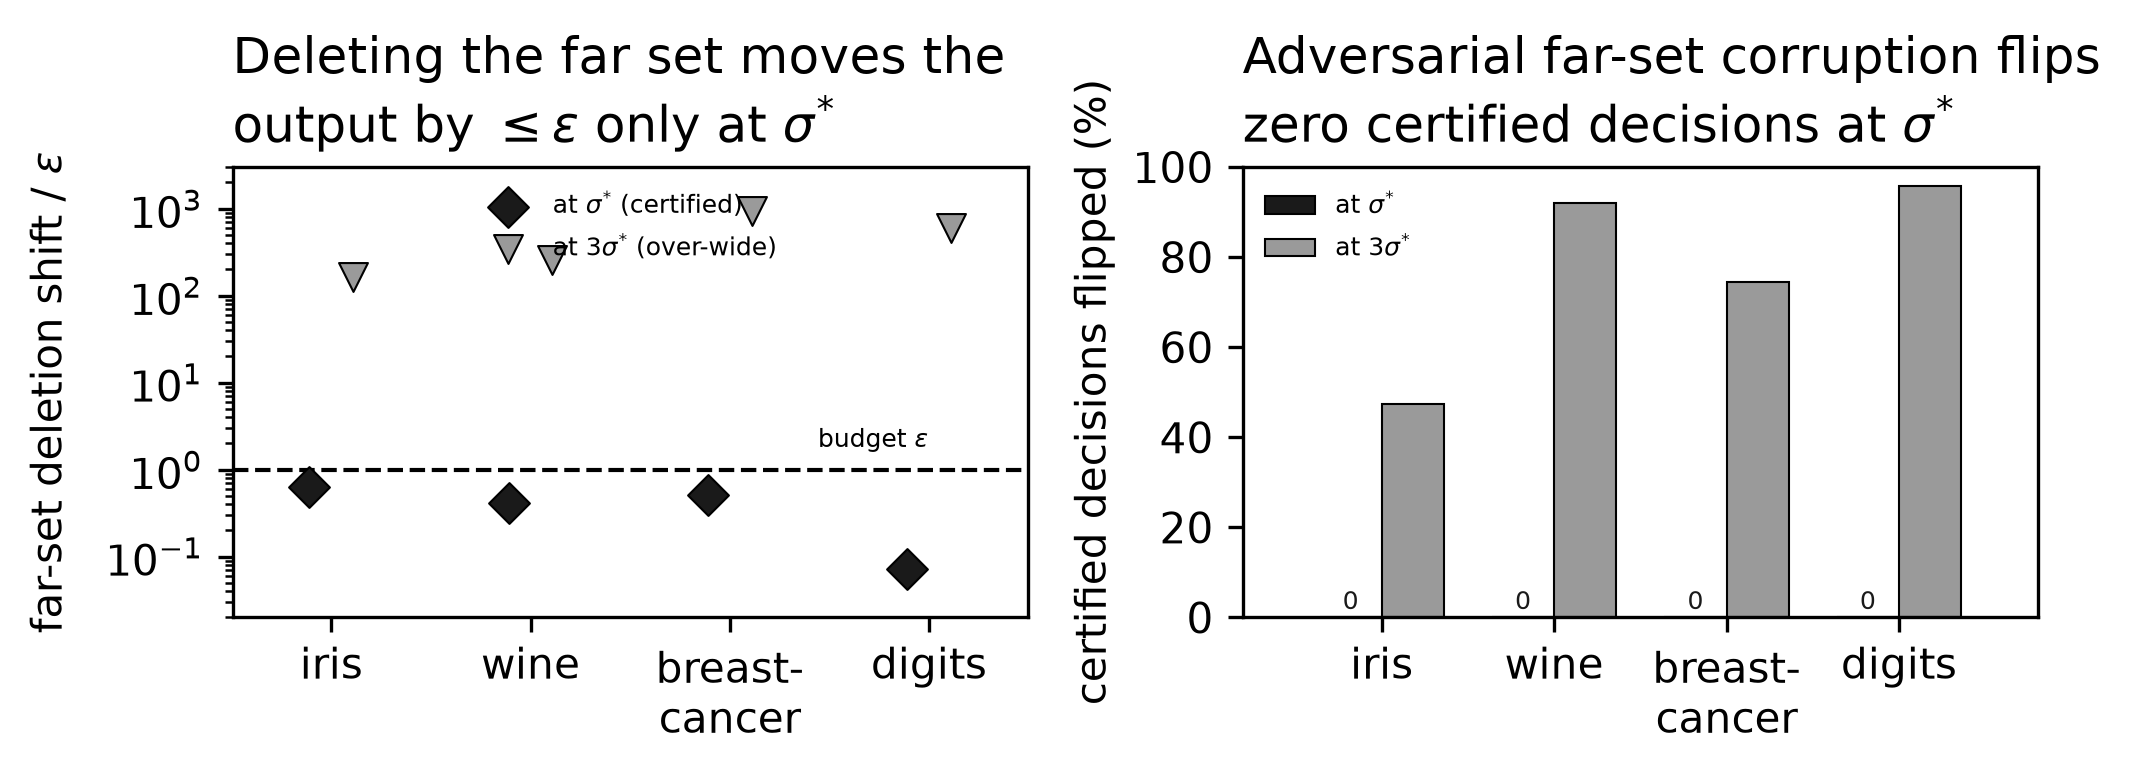
\includegraphics[width=\linewidth]{figs/fig_86d51bd8-18e.png}
\caption{\textbf{Certified output locality.} (a) Deleting all far sources moves the output by at most $\varepsilon$ at $\sstar$ on all four datasets; $3\sstar$ overshoots by two to three orders of magnitude. (b) Under admissible far-set corruption, certified-stable decisions do not flip at $\sstar$, versus $47$--$96\%$ at $3\sstar$.}
\label{fig:locality}
\end{figure}

\subsection{Calibration holds where bandwidth heuristics do not}\label{sec:flagship}

We build Parzen-vote fields on frozen ResNet-18, ResNet-50 and ViT-B/16 features of CIFAR-100, fixing $\varepsilon=0.05$ and using no labels to compute $\sstar$ (Methods). The naive single-source bandwidth overshoots the aggregate budget by $4.9\times10^3$--$1.0\times10^4$ and joins $97$--$100\%$ of centres into one component. The certified frontier holds tail/$\varepsilon$ to $0.08$--$0.16$, reduces the largest component to $4$--$7\%$, and reaches accuracies of $56.6\%$, $51.0\%$ and $72.5\%$, within $0.6$, $5.1$ and $0.5$ points of the labelled grid-search optima (Fig.~\ref{fig:multibb}). Across five re-samples, its accuracy varies by at most $0.3$ points.

The median and $k$-nearest-neighbour heuristics select bandwidths $3.6$--$6\times$ larger than $\sstar$, driving tail/$\varepsilon$ to approximately $10^5$ and losing $9$--$26$ accuracy points. Classical density selectors also miss the budget because they optimise density error rather than interference. These comparisons do not imply that the selectors fail at their own objectives; they show that predictive or density fit does not certify aggregate locality. A direct label-free bisection of the measured mean tail finds a bandwidth $1.07$--$1.11\times\sstar$, but its 99th-percentile tail exceeds the budget by $1.6$--$2.3\times$; the closed-form frontier trades this small bandwidth increment for a conservative certificate. A hard-truncated Gaussian, which forces exact zero far mass by clipping the kernel at radius $d$, is the natural same-objective locality baseline; at its labelled-grid bandwidth it reaches $55.8\%$ (against $\sstar$'s $56.6\%$) yet agrees with the smooth field on only $89\%$ of decisions, so discontinuous compact support buys exact locality at a cost in accuracy and decision consistency that the smooth $\varepsilon$-bounded field avoids (SI Note~3).

The near sources are $25$--$47\times$ enriched for the query class relative to chance, although they are not always a majority. Thus the radius identifies a meaningful local vote, but the theorem guarantees which region supplies the decision, not that the decision is correct. Sweeping $\varepsilon$ and the radius percentile changes the realised $\sstar$ by only $1.34$--$1.41\times$ and leaves the certified tail in budget (SI Note~14).

\begin{figure}[t]
\centering
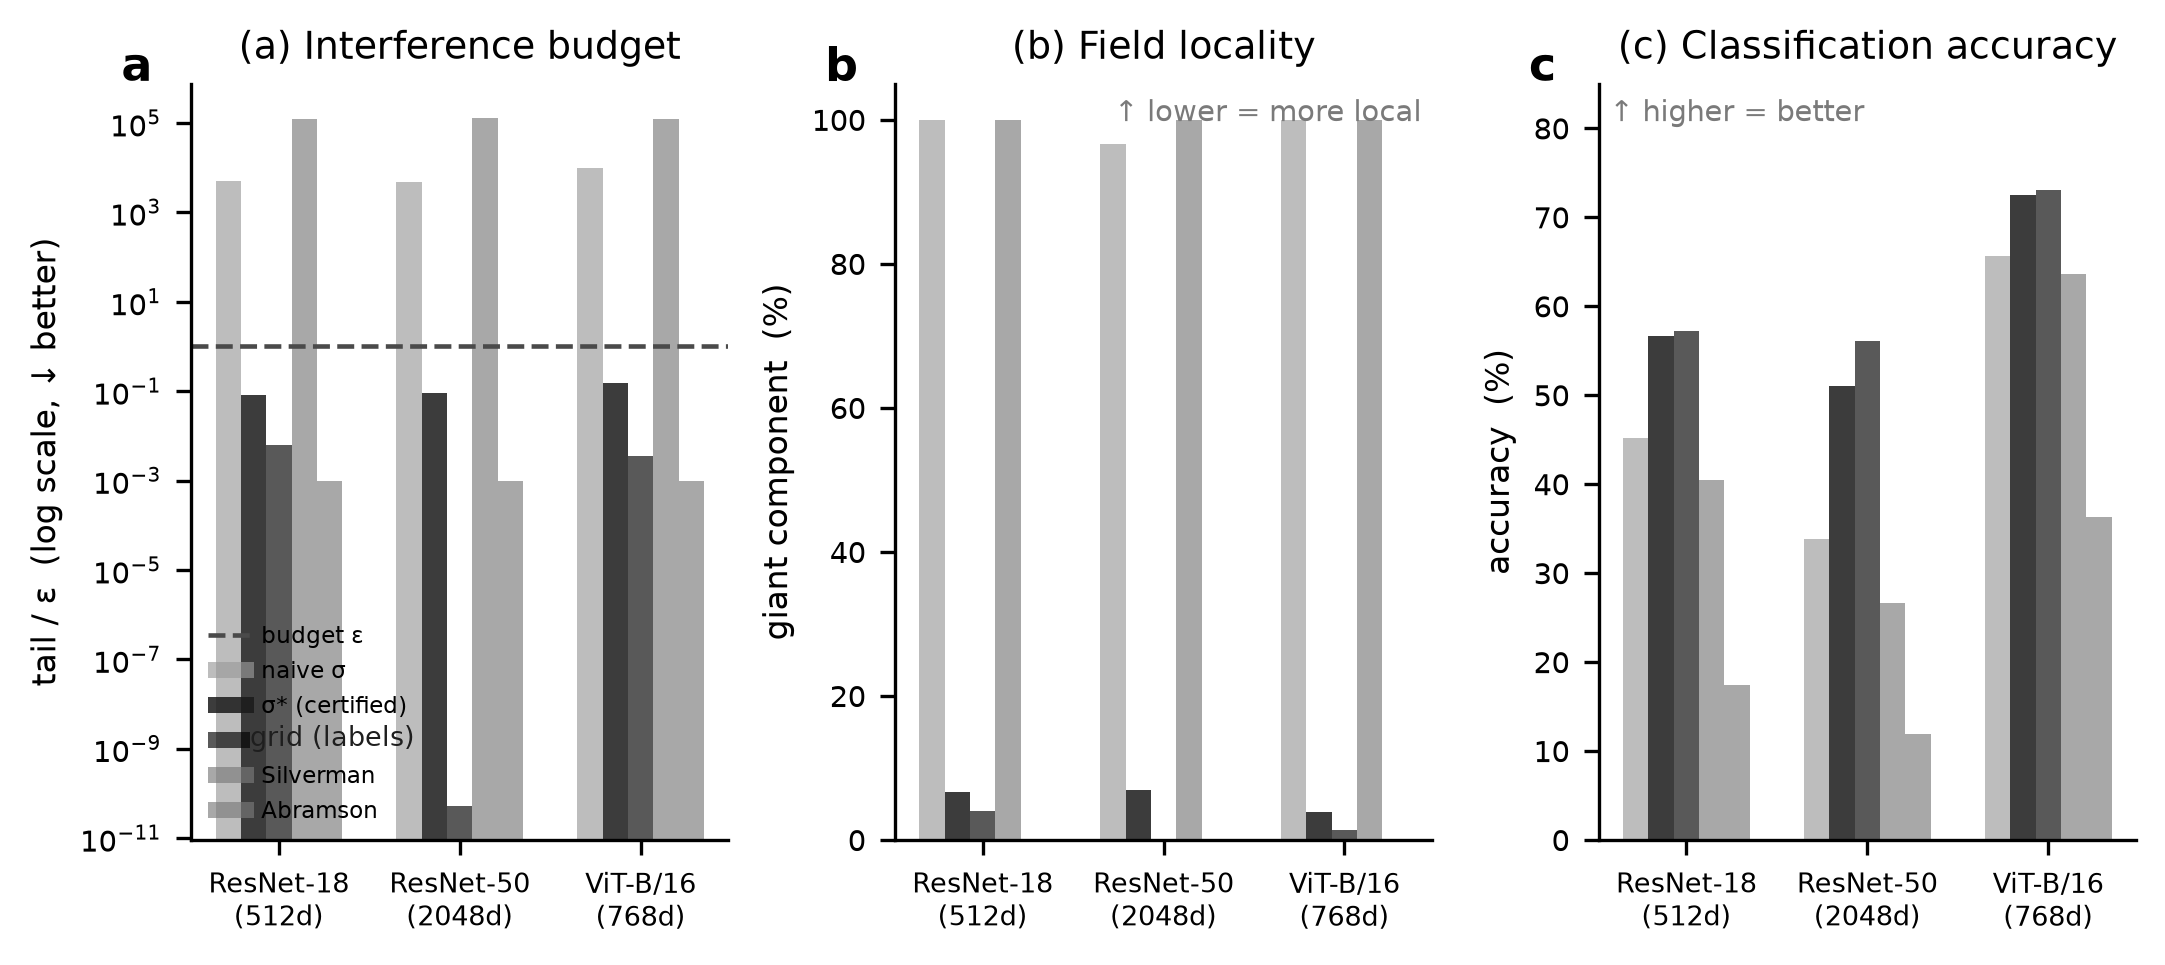
\includegraphics[width=\linewidth]{figs/fig_bbb3a079-7e7.png}
\caption{\textbf{Certified calibration on three frozen backbones.} (a) Only $\sstar$ holds the interference budget; naive and density bandwidths overshoot by $10^3$--$10^5\times$. (b) Those bandwidths collapse the field into one component, whereas $\sstar$ preserves locality. (c) $\sstar$ approaches labelled grid-search accuracy without labels.}
\label{fig:multibb}
\end{figure}

The same pattern reproduces beyond vision. On DBpedia, AG-News, Yahoo-Answers and Covertype, $\sstar$ holds tail/$\varepsilon<1$ while the naive bandwidth overshoots by $3.6\times10^2$--$2.3\times10^3$ (Fig.~\ref{fig:modality}). It matches labelled grid search within $0.9$ points on the three text sets and trails by $5.8$ points on low-dimensional Covertype. On four smaller public datasets it matches the labelled optimum within about two points on three of four. The principle also extends beyond the Gaussian: for the Laplace kernel, $\sstar=d/\ln(A/\varepsilon)$ holds tail/$\varepsilon$ to $0.16$--$0.24$ and remains within $0$--$2.8$ accuracy points of labelled search (SI Note~3).

\begin{figure}[t]
\centering
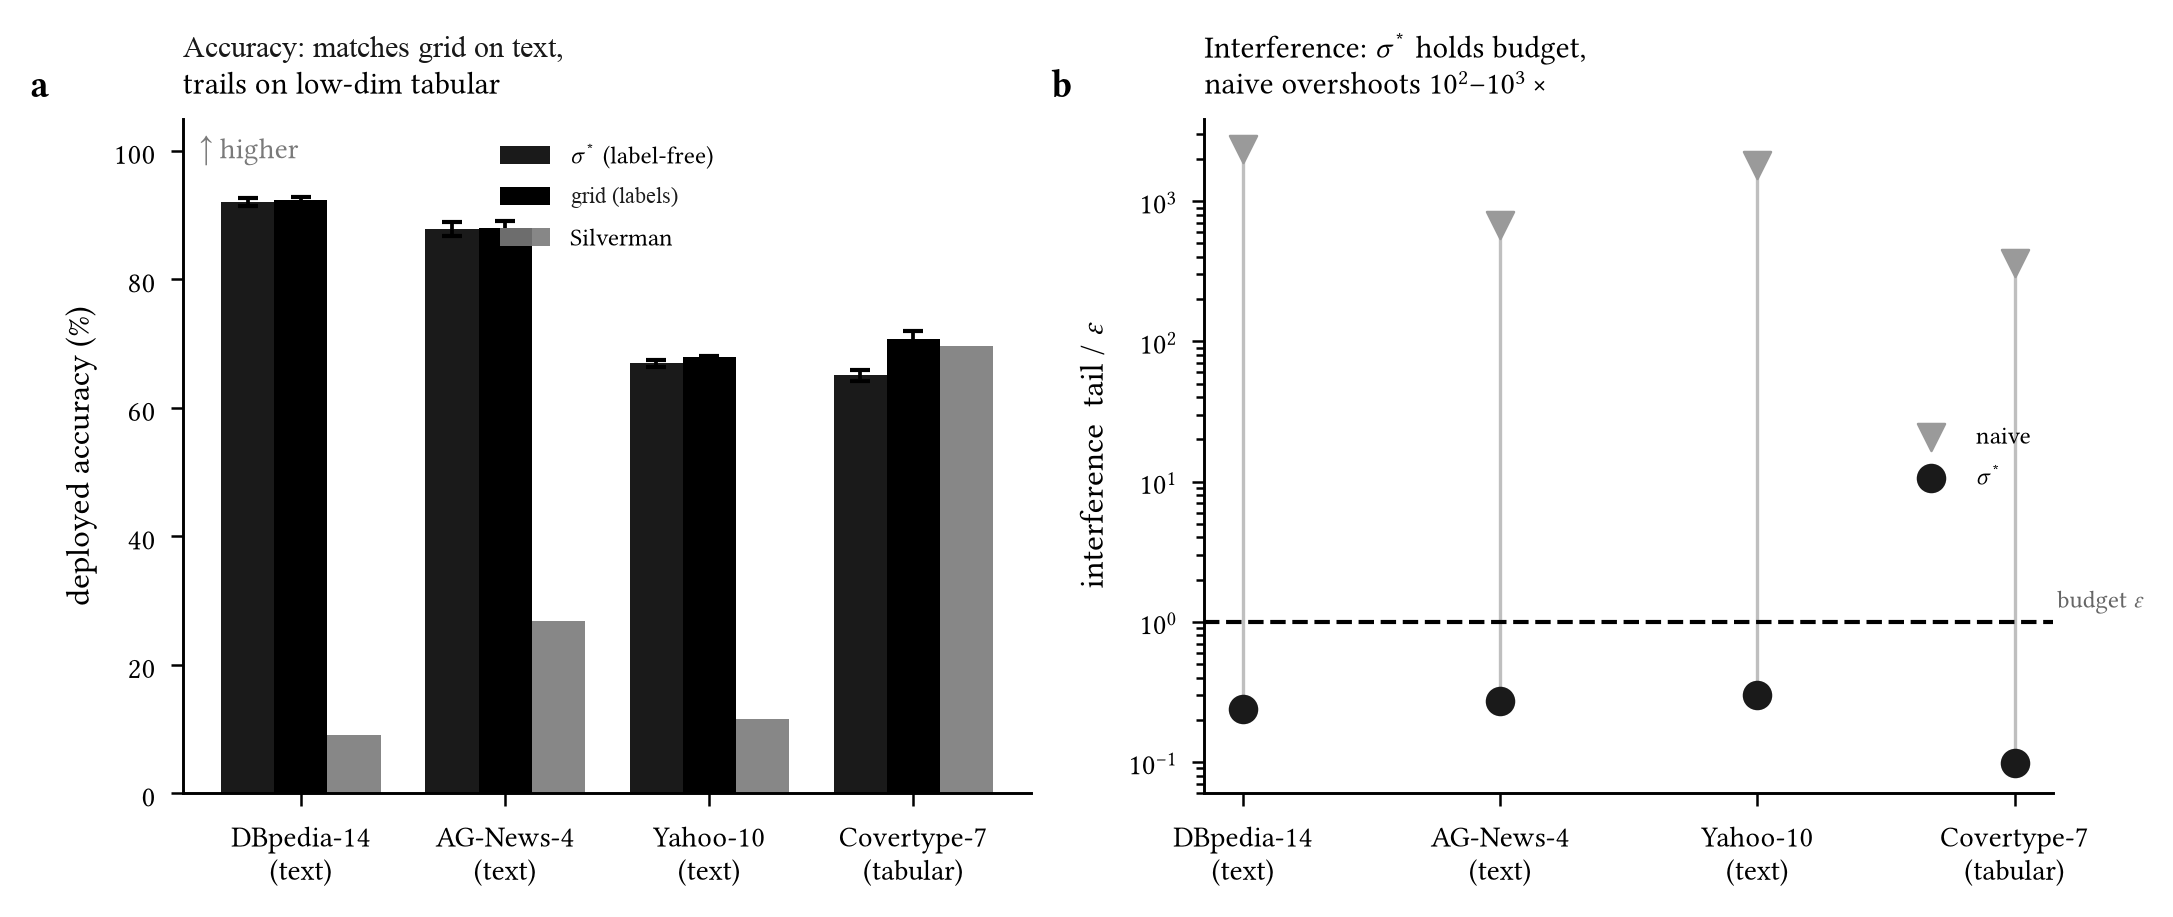
\includegraphics[width=\linewidth]{figs/fig_e3209e61-9ae.png}
\caption{\textbf{Cross-modal replication.} (a) $\sstar$ matches labelled grid search on three text datasets and trails on low-dimensional tabular data; error bars are $\pm1$ s.d. over five seeds. (b) It holds the budget on every corpus, while the naive bandwidth overshoots by two to three orders of magnitude.}
\label{fig:modality}
\end{figure}

\subsection{Re-calibration follows memory density}\label{sec:grow}

Because $A$ is measured rather than fitted, calibration can be repeated when a field changes. We grow each frozen feature field from $3$ to $120$ examples per class, comparing $\sstar$ re-certified at every stage with a labelled grid-search bandwidth fixed on the initial sparse field. As density increases, $\sstar$ shrinks and holds tail/$\varepsilon\approx0.1$ (Fig.~\ref{fig:grow}). The frozen bandwidth reaches $502\times$ budget on ResNet-18 and $3{,}865\times$ on ViT-B/16; re-calibration improves accuracy by $7.0$ and $6.1$ points, respectively. ResNet-50 is the boundary case: its frozen bandwidth reaches only about $2\times$ budget, while $\sstar$ gains $3.2$ points. The radius itself drifts by only $1\%$ over the $40\times$ densification; the dominant change is the measured mass.

This result is adaptivity, not dominance over fresh labelled tuning. Re-certified $\sstar$ tracks a per-stage labelled oracle closely on ResNet-18 and ViT-B/16 and trails it by approximately four points on ResNet-50. It also follows density rather than field size: adding classes at fixed density barely changes the geometry, and the frozen bandwidth then stays in budget and ties $\sstar$. The null fixes the scope of the growing-memory claim. Recomputing the median and $k$-nearest-neighbour scales label-free at every density stage, so that all label-free methods receive the updated geometry, does not help: both overshoot the budget by four to five orders of magnitude at every stage, confirming that adapting the scale is not the same as holding the interference budget (SI Note~15).

\begin{figure}[t]
\centering
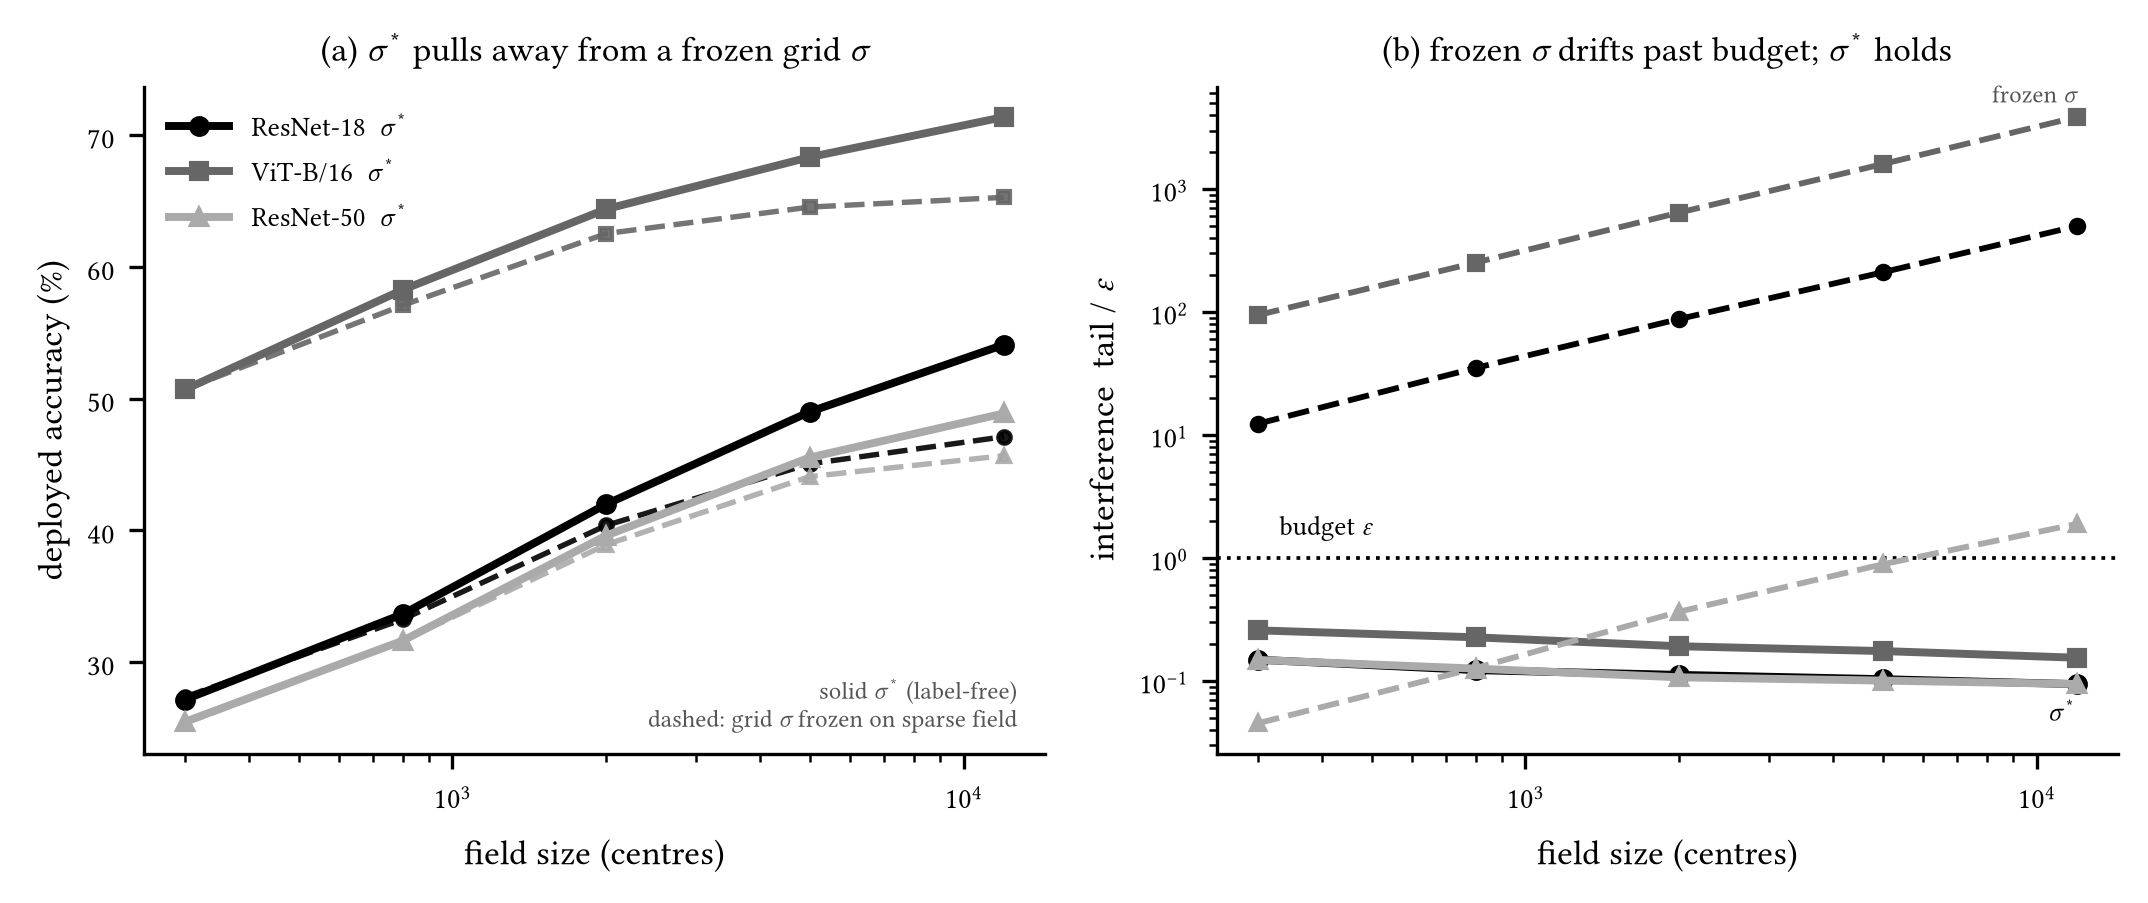
\includegraphics[width=\linewidth]{figs/fig_97f5129f-934.png}
\caption{\textbf{Re-calibration under densification.} A labelled bandwidth is fixed on the sparse field; $\sstar$ is re-measured without labels. (a) $\sstar$ tracks a per-stage labelled oracle and gains $3.2$--$7.0$ accuracy points over the frozen bandwidth at full density. (b) The frozen bandwidth drifts beyond budget while $\sstar$ remains near $0.1\varepsilon$.}
\label{fig:grow}
\end{figure}

\subsection{Normalised readouts inherit a Gibbs certificate}\label{sec:reach}

Additive bounds do not directly control a normalised readout because deleting far sources changes its denominator. Let $p_i=e^{-E_i/\tau}/\sum_j e^{-E_j/\tau}$, let $E_0=\min_iE_i$, and define the far set by an energy gap $E_i\ge E_0+\Delta$. If $D_q^{\mathcal{F}}(\tau)$ is the Hill number of the anchor-shifted far weights, the output-relevant far probability mass $m_{\mathcal{F}}=\sum_{i\in\mathcal{F}}p_i$ obeys a direct certificate.

\begin{theorem}[Gibbs far-mass certificate]\label{thm:gibbs}
For every $q\ge2$,
\begin{equation}
m_{\mathcal{F}}(\tau)\le D_q^{\mathcal{F}}(\tau)e^{-\Delta/\tau}.
\end{equation}
Measure $D_{q,0}=D_q^{\mathcal{F}}(\tau_0)$ once and set
\begin{equation}
\tau_{\mathrm{cert}}=\min\!\left(\tau_0,\frac{\Delta}{\ln(D_{q,0}/\varepsilon)}\right).
\end{equation}
Then $m_{\mathcal{F}}(\tau_{\mathrm{cert}})\le\varepsilon$.
\end{theorem}

For a normalised output $O=\sum_i p_i u_i$ with $\lVert u_i\rVert\le B$, deleting the far set and renormalising changes the output by at most $2B\varepsilon$ (SI Note~10). Unlike the additive form, the Gibbs bound has no source-amplitude factor: it controls the probability mass read by the softmax directly. The theorem therefore applies exactly to a prototypical network~\cite{snell2017} with $E_i=\lVert f(x)-c_i\rVert^2$ and to attention with $E_i=-\langle q,k_i\rangle$.

On a conv-4 ProtoNet, the reference far mass is $0.080$ at $\tau_0=1$. For approximately $30\%$ of queries the naive inverted temperature would be warmer than $\tau_0$; the minimum in Theorem~\ref{thm:gibbs} is therefore essential. The certified temperature reduces far mass to means of $0.015$ for $q=2$ and $0.017$ for $q=\infty$, with maximum $0.0476<\varepsilon$ over $7{,}200$ queries (Fig.~\ref{fig:gibbs}a). A separate additive-field experiment confirms the bounded-weight case: the unnormalised prototype tail is $0.25\varepsilon$ at $\sstar$ over $12{,}000$ queries (SI Note~8).

\begin{figure*}[t]
\centering
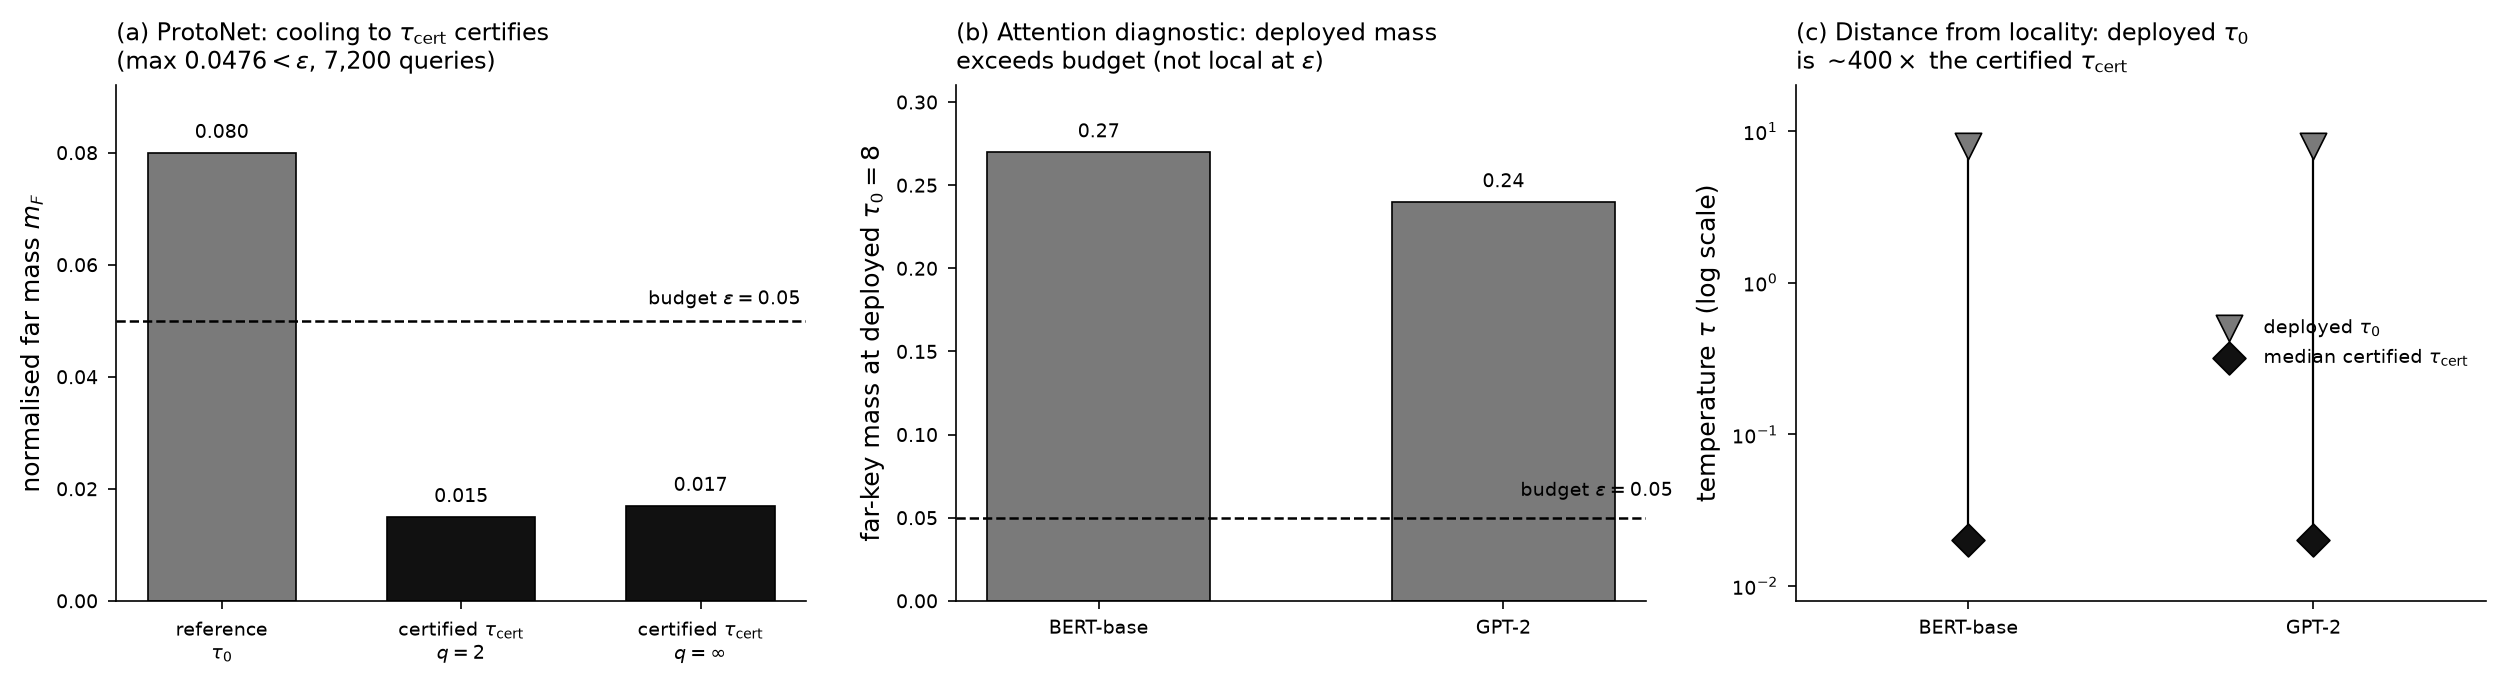
\includegraphics[width=0.98\linewidth]{figs/fig_gibbs_operational.png}
\caption{\textbf{The operational Gibbs certificate.} (a) A conv-4 prototypical network: cooling from the reference temperature $\tau_0$ to the certified $\tau^*$ pulls the normalised far mass from $0.080$ below the budget $\varepsilon=0.05$ (means $0.015$ for $q=2$, $0.017$ for $q=\infty$; maximum $0.0476<\varepsilon$ over $7{,}200$ queries). (b) Pretrained attention is the diagnostic boundary: at the deployed $\tau_0=\sqrt{d_k}=8$ the far-key mass is $0.27$ (BERT-base) and $0.24$ (GPT-2), above budget, so deployed attention is not concentrated on its designated near-key set at $\varepsilon=0.05$. (c) The per-query certified temperatures have median $\approx0.02$, roughly $400\times$ colder than deployment: meeting the budget would require radically sharper attention, a diagnostic scale rather than a deployable retuning.}
\label{fig:gibbs}
\end{figure*}

Pretrained attention provides the diagnostic boundary case (Fig.~\ref{fig:gibbs}b,c). With the near set defined by the top-decile logits, so that ``local'' means concentration on the designated high-logit key set rather than positional proximity, BERT-base and GPT-2 at the deployed temperature $\tau_0=\sqrt{d_k}=8$ carry far-key mass $0.27$ and $0.24$: bounded and computable, but deployed attention is not concentrated on its designated near-key set at $\varepsilon=0.05$. The per-query certified temperatures have median approximately $0.02$, showing that meeting this budget would require radically sharper attention. These are diagnostic temperatures, not a deployable global retuning. The pointwise Gibbs bound holds across approximately $66{,}000$ query-heads. Propagating the measured head masses through the value and output projections also bounds full-layer deletion perturbation; on BERT the actual perturbation is $12$--$28\%$ of layer-output norm and the weight-norm bound is conservative by about $50\times$ (SI Note~11). The additive Gaussian representation~\cite{tsai2019,choromanski2021}, valid only at a fixed temperature, is given separately in SI Note~7.

\section{Discussion}

The Resolution Calibration Principle changes the role of bandwidth or temperature. Rather than selecting resolution only for predictive fit, it derives the largest operating scale certified to satisfy a locality budget. For additive fields, one measured effective mass gives a closed-form frontier; the same bound controls decision stability, deletion and abstention. Re-measurement adapts the certificate as memory density changes, while the Gibbs form extends it to normalised prototype and attention readouts. The experiments show both outcomes a certificate should expose: ProtoNet can be operated within budget, whereas deployed transformer attention is measurably far from it.

The objective distinguishes this work from bandwidth selectors that minimise density error or predictive loss~\cite{silverman1986,scott1992,sheather1991,botev2010,gpml}; such rules can be statistically appropriate while leaving interference uncontrolled. Distance heuristics~\cite{garreau2017,zelnikmanor2004} set a geometric scale but omit the effective-mass safety factor. Direct tail bisection targets the same mean interference empirically, but lacks the one-shot conservative envelope and can leave upper-quantile queries over budget. Conformal and selective prediction~\cite{vovk2005,angelopoulos2023,geifman2017} address complementary uncertainty questions; here an unlabelled conformal sample calibrates future-query coverage of a geometric mass rather than prediction error. The deletion bound also connects to unlearning and influence attribution~\cite{ginart2019,koh2017}, but certifies output sensitivity only under the stated bounded-weight and admissibility assumptions. Architectural locality -- sparse or windowed attention~\cite{child2019,beltagy2020} and hash-bucketed retrieval~\cite{kitaev2020,andoni2008} -- imposes a fixed near/far structure by design; the certificate here instead measures whether an unmodified field already respects an interference budget, and at what resolution. Kernel-based attribution~\cite{yeh2018} decomposes a prediction into per-source contributions but does not bound the aggregate far-set influence that the certificate controls.

Three limits delimit the claim. The principle requires a meaningful near/far separation and is silent for pure density recovery where every sample is intended to contribute. It calibrates interference, not accuracy; accuracy gains appear in dense growing fields, whereas fixed low-density fields show parity. Finally, one-shot conservativeness assumes fixed source amplitudes and a fixed radius as bandwidth varies. Representations whose coefficients or geometry co-adapt require those quantities to be re-certified. The construction is radial only relative to the chosen geometry: the same proof applies to any frozen scale-independent dissimilarity, including fixed Mahalanobis and graph-derived distances (SI Note~3), whereas jointly learned geometries require re-certification. This suggests the next step: incorporate the differentiable $D_2$ tail into end-to-end training so that representation and resolution become local by construction rather than only certified after fitting.

\section{Methods}

\paragraph{Construction.} For each backbone---ResNet-18 ($512$-d), ResNet-50 ($2048$-d), and ViT-B/16 ($768$-d), all ImageNet-pretrained and frozen---we extract the penultimate features of CIFAR-100 and build a correction field of $20{,}000$ balanced kernels ($200$ per class) over the training features, classified by a kernel-weighted (Parzen) vote. The locality radius $d$ is the tenth percentile of pairwise centre distances---pure geometry, no labels. We fix $\varepsilon=0.05$ a priori and compare the naive single-interferer rule $\sigma_{\mathrm{pair}}=d/\sqrt{2\ln(1/\varepsilon)}$, the certified frontier $\sstar$, and a labelled grid search over a $30$-point log-spaced grid. We also run classical density bandwidths, the median heuristic and a $k$-nearest-neighbour scale.

\paragraph{Computing $\sstar$.} Four steps require no labels: (1) fix $\varepsilon$ and set $d$ to the tenth percentile of pairwise centre distances; (2) form $\sigma_{\mathrm{pair}}=d/\sqrt{2\ln(1/\varepsilon)}$; (3) measure $A=V_{\max}\Neff$ at $\sigma_{\mathrm{pair}}$, averaging the far-mask participation ratio over queries; and (4) return $\sstar=d/\sqrt{2\ln(A/\varepsilon)}$. Proposition~\ref{prop:conserv} makes this measurement conservative. Quantile and conformal variants replace the mean mass by the required upper order statistic. Full grids, seeds and growing-field and modality protocols are in SI Note~15.

\paragraph{Normalised fields.} For each query, the Gibbs experiments measure $D_q^{\mathcal{F}}$ at the model's reference temperature $\tau_0$ and deploy or diagnose the pointwise $\tau_{\mathrm{cert}}$ of Theorem~\ref{thm:gibbs}. Attention uses the top-decile-logit keys as the near anchor and the remainder as the far set. The ProtoNet uses squared query--prototype distance, with the far gap measured from the nearest prototype. Architectural, sampling and numerical details are in SI Notes~7--11.

\paragraph{Hard-truncation comparator.} As a same-objective locality baseline we run a hard-truncated Gaussian $K^{\mathrm{trunc}}_\sigma(r^2)=K_\sigma(r^2)\mathbf{1}\{r\le d\}$, whose bandwidth is chosen by the same labelled oracle grid. It has exact zero far mass by construction, so it changes the readout rather than calibrating it. We compare accuracy and decision agreement with the smooth field; full results in SI Note~13.

\paragraph{Frozen-geometry stress test.} To probe the frozen-geometry corollary (SI Note~3) we build controlled anisotropic-Gaussian, two-moons and densification settings and run RCP under isotropic-Euclidean, frozen global-Mahalanobis and frozen out-of-sample graph-geodesic dissimilarities, holding each geometry fixed during calibration. We report tail budget, per-query violation rate and decision accuracy in SI Note~14.

\paragraph{Reproducibility.} The full computational specification, proofs, supplementary displays and released outputs are in the Supplementary Information and repository. Proofs of the additive frontier, one-shot monotonicity, decision and deletion corollaries, R\'enyi family, Gibbs certificate and conformal query certificate are given in SI Notes~1--15.

\paragraph{Data and code availability.} All experiment scripts and released result files are available at \texttt{github.com/negulescu42/sigma-star}, with fixed seeds and the exact bandwidth grid for each experiment.

\paragraph{Author contributions.} R.N. conceived the resolution-calibration framing, developed the empirical and machine-learning programme, and carried out the transformer, prototype-network and re-calibration experiments. M.T. performed the mathematical audit and contributed the vector $\ell_1$ decision certificate and the sharpened statements of the additive results. C.B. developed the analytic core, including Propositions~\ref{prop:frontier}--\ref{prop:conserv}, Theorem~\ref{thm:stable}, Corollary~\ref{cor:locality}, and the R\'enyi, Gibbs and conformal extensions. All authors reviewed and approved the manuscript.

\begin{thebibliography}{99}
\small
\bibitem{silverman1986} B. W. Silverman. \emph{Density Estimation for Statistics and Data Analysis.} Chapman \& Hall, 1986.
\bibitem{scott1992} D. W. Scott. \emph{Multivariate Density Estimation.} Wiley, 1992.
\bibitem{sheather1991} S. J. Sheather, M. C. Jones. \emph{A Reliable Data-Based Bandwidth Selection Method for Kernel Density Estimation.} J. R. Stat. Soc. B 53:683--690, 1991.
\bibitem{botev2010} Z. I. Botev, J. F. Grotowski, D. P. Kroese. \emph{Kernel Density Estimation via Diffusion.} Ann. Statist. 38(5):2916--2957, 2010.
\bibitem{gpml} C. E. Rasmussen, C. K. I. Williams. \emph{Gaussian Processes for Machine Learning.} MIT Press, 2006.
\bibitem{vovk2005} V. Vovk, A. Gammerman, G. Shafer. \emph{Algorithmic Learning in a Random World.} Springer, 2005.
\bibitem{angelopoulos2023} A. N. Angelopoulos, S. Bates. \emph{Conformal Prediction: A Gentle Introduction.} Found. Trends Mach. Learn. 16(4):494--591, 2023.
\bibitem{geifman2017} Y. Geifman, R. El-Yaniv. \emph{Selective Classification for Deep Neural Networks.} NeurIPS, 2017.
\bibitem{garreau2017} D. Garreau, W. Jitkrittum, M. Kanagawa. \emph{Large Sample Analysis of the Median Heuristic.} arXiv:1707.07269, 2017.
\bibitem{zelnikmanor2004} L. Zelnik-Manor, P. Perona. \emph{Self-Tuning Spectral Clustering.} NeurIPS, 2004.
\bibitem{rippa1999} S. Rippa. \emph{An Algorithm for Selecting a Good Value for the Parameter $c$ in Radial Basis Function Interpolation.} Adv. Comput. Math. 11:193--210, 1999.
\bibitem{ginart2019} A. Ginart et al. \emph{Making AI Forget You: Data Deletion in Machine Learning.} NeurIPS, 2019.
\bibitem{koh2017} P. W. Koh, P. Liang. \emph{Understanding Black-box Predictions via Influence Functions.} ICML, 2017.
\bibitem{snell2017} J. Snell, K. Swersky, R. Zemel. \emph{Prototypical Networks for Few-shot Learning.} NeurIPS, 2017.
\bibitem{tsai2019} Y.-H. H. Tsai et al. \emph{Transformer Dissection: A Unified Understanding of Transformer's Attention via the Lens of Kernel.} EMNLP, 2019.
\bibitem{choromanski2021} K. Choromanski et al. \emph{Rethinking Attention with Performers.} ICLR, 2021.
\bibitem{hill1973} M. O. Hill. \emph{Diversity and Evenness: A Unifying Notation and Its Consequences.} Ecology 54(2):427--432, 1973.
\bibitem{renyi1961} A. R\'enyi. \emph{On Measures of Entropy and Information.} Proc. Fourth Berkeley Symp. on Math. Stat. and Prob., Vol. 1, pp. 547--561, 1961.
\bibitem{child2019} R. Child, S. Gray, A. Radford, I. Sutskever. \emph{Generating Long Sequences with Sparse Transformers.} arXiv:1904.10509, 2019.
\bibitem{beltagy2020} I. Beltagy, M. E. Peters, A. Cohan. \emph{Longformer: The Long-Document Transformer.} arXiv:2004.05150, 2020.
\bibitem{kitaev2020} N. Kitaev, {\L}. Kaiser, A. Levskaya. \emph{Reformer: The Efficient Transformer.} ICLR, 2020.
\bibitem{andoni2008} A. Andoni, P. Indyk. \emph{Near-Optimal Hashing Algorithms for Approximate Nearest Neighbor in High Dimensions.} Commun. ACM, 51(1):117--122, 2008.
\bibitem{yeh2018} C.-K. Yeh, J. Kim, I. E. H. Yen, P. Ravikumar. \emph{Representer Point Selection for Explaining Deep Neural Networks.} NeurIPS, 2018.
\end{thebibliography}

\end{document}